\section{Introduction}
\label{sec:intro}
In recent years, there has been an extensive amount of work
on the verification of \emph{parameterized systems},
e.g.~\cite{BJNT:rmc,KMMPS2001,AJNO:simple,BLW03,BHV04}.
%
Typically, a parameterized system consists of an arbitrary number
of finite-state processes organized in a linear array.
%
The task is to perform \emph{parameterized verification}, i.e.\
to verify correctness of the system regardless
of the number of processes inside the system.
%
Examples of parameterized systems include 
mutual exclusion algorithms, bus protocols, 
telecommunication protocols, multi-threaded programs, and cache coherence
protocols.
% 
This work aims at extending the paradigm of parameterized verification
in order to verify systems which operate on tree-like architectures.
%
More precisely, we consider analysis of safety properties for
\emph{parameterized tree systems}.
%
Such a system consists of an arbitrary number
of finite-state processes which operate on a tree-like architecture.
%
%
Examples of parameterized tree systems include 
several interesting  protocols such as the percolate
protocol~\cite{KMMPS2001},the Tree-arbiter protocol~\cite{ABHQR:BDD:POM}, 
and the IEEE 1394 Tree identity protocol~\cite{ieee:1394}.
% 

One of the most prominent techniques which have been used
for verification of parameterized tree systems is that of \emph{tree regular model 
checking}~\cite{DLS01,ABMO:tree,KMMPS2001,BT02,rmc:tree:simulation:journal}. 
%
In tree regular model checking, configurations (states) of the system are represented
by trees, sets of configurations by tree automata, and transitions by tree
automata operating on pairs of trees, i.e.\ tree transducers. 
%
Safety properties can be checked through performing
reachability analysis, which amounts to applying
the tree transducer relation iteratively to the set of initial configurations.
%
The main problem with transducer-based techniques, such as the ones mentioned above, is that they
are very heavy and usually rely on several layers of computationally
expensive automata-theoretic constructions; in many cases
severely limiting their applicability.
%

In this paper, we propose a light-weight approach to parameterized tree verification
which, in addition to its simplicity, also yields a much more efficient implementation
than tree regular model checking.
%
In our method, a configuration of the system is represented by a tree over 
a finite alphabet, where elements of the alphabet represent the local states of 
the individual processes.
%
The behaviour of the system is induced by a set of
rewriting rules which describe how the processes perform transitions.
%
A transition performed by a process is
conditioned by the current local state of the process and 
possibly the local states of neighboring  processes, i.e.\ the parent and children processes.
%
The  transition may change the states of all involved processes. (see Figure~\ref{fig:intro}).
%

\begin{figure}
\centering
  \begin{tikzpicture}[show background rectangle]
    \tikzstyle{level 1}=[sibling distance=2cm,level distance=1.2cm]
    \tikzstyle{every node}=[draw,rounded corners,minimum width=1cm]
    \node {$\state_1$ / $\state'_1$}
    child {node{$\state_2$ / $\state'_2$}}
    child {node{$\state_3$ / $\state'_3$}}
    ;
  \end{tikzpicture}
  \caption{A typical transition rule where a process and its two children change state from 
    $\state_1,\state_2,\state_3$ to $\state'_1,\state'_2,\state'_3$, respectively.}
  \label{fig:intro}
\end{figure}
%

Observe that the set of configurations is infinite since we are dealing
with trees of an arbitrary size.
%
In fact, parameterized verification amounts to
analyzing an infinite family of systems;
namely one for each size of the system and one for each tree of that particular size.

\ignore{
\noindent
\begin{minipage}{0.55\textwidth}
\setlength{\parindent}{1em}
\noindent%
A transition performed by a process is
conditioned by the current local state of the process and 
possibly the local states of neighboring  processes, i.e.\ the parent and children processes.
%
The  transition may change the states of all involved processes.% (see Figure~\ref{fig:intro}).
%

Observe that the set of configurations is infinite since we are dealing
with trees of an arbitrary size.
%
In fact, parameterized verification amounts to
analyzing an infinite family of systems;
namely one for each size of the system and one for each tree of that particular size.
\end{minipage}
%
% Right part
%
%\framebox{%
\hfill%
\begin{minipage}{0.4\textwidth}
\begin{center}
  \begin{tikzpicture}[show background rectangle]
    \tikzstyle{level 1}=[sibling distance=2cm,level distance=1.2cm]
    \tikzstyle{every node}=[draw,rounded corners,minimum width=1cm]
    \node {$\state_1$ / $\state'_1$}
    child {node{$\state_2$ / $\state'_2$}}
    child {node{$\state_3$ / $\state'_3$}}
    ;
  \end{tikzpicture}

  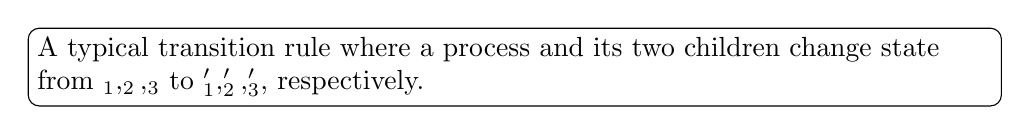
\begin{tikzpicture}
    \node[text width=\textwidth] {A typical transition rule where a process and its two children change state from 
      $\state_1,\state_2,\state_3$ to $\state'_1,\state'_2,\state'_3$, respectively.};
  \end{tikzpicture}
\end{center}
\end{minipage}
%}%
}

The main idea of our method is to consider a transition relation
which is an over-approximation of the one induced by the tree parameterized system.
%
To do so, we modify the semantics of the transition rules, such that a rule is applied
to a node and two nodes in its left and right subtrees (rather than its
left and right children).
%
The approximate transition system obtained in this manner is \emph{monotonic}
with respect to the tree embedding relation on configurations (larger configurations
are able to simulate smaller ones).
%
Since the approximate transition relation is monotonic, it can be analyzed using
 symbolic backward reachability algorithm based on a generic method
introduced in~\cite{Parosh:Bengt:Karlis:Tsay:general}.
%
An attractive feature of this algorithm is that it operates
on sets of configurations which are upward closed with respect
to the tree embedding relation.
%
This allows an efficient symbolic representation of upward sets of configurations,
since such a set can be represented by (the finite set of) its minimal elements.
%
Since the minimal elements are trees, reachability analysis can be performed by computing
predecessors of trees, which is much simpler and more efficient
than applying transducer relations on general tree regular languages.
%
Also, as a side effect, the analysis of the approximate model is
guaranteed to terminate.
%
This follows from the fact that the embedding relation on configurations (trees)
is a \emph{well quasi-ordering} by Kruskal's theorem~\cite{kruskal}.
%
The whole verification process is fully automatic since both
the approximation and the reachability analysis are carried out
without user intervention.
%
Observe that if the approximate transition system satisfies a 
safety property then we can safely conclude that
the original system satisfies the property too.

Based on the method,
we have implemented a prototype  which 
works well on several tree-based protocols such as 
the percolate, leader election, Tree-arbiter, and the IEEE 1394 Tree identity protocols.
% 

\paragraph{\bf Outline}
%
In the next section, we give some preliminaries on trees.
%
In Section~\ref{sec:parsys}, we define the basic model of parameterized tree systems.
%
In Section~\ref{sec:ts}, we describe the induced transition system and in Section~\ref{sec:approx}, 
we define the over-approximated transition system on which we run our algorithm.
%
We present a generic scheme for deciding reachability of upward closed sets in Section~\ref{sec:scheme}, 
and we show how to instantiate it on our model in Section~\ref{sec:alg}.
%
In Section~\ref{sec:exp}, we report our experimental results on several tree protocols.
%
Section~\ref{sec:conc} concludes the paper and gives direction for future works.
%
Some proofs as well as the details of the case studies can be found in~\cite{it:2008-010}.
%
